\input /users/davidmcallester/icloud/tex/SlidePreamble
\input /users/davidmcallester/icloud/tex/preamble

\begin{document}

{\Huge

  \centerline{\bf TTIC 31230, Fundamentals of Deep Learning}
  \bigskip
  \centerline{David McAllester, Autumn 2023}
  \vfill
  \vfill
  \centerline{\bf Variational Auto-Encoders (VAEs)}
  \vfill
  \vfill

\slide{Generative AI: Autoregression and GANs}

For an autoregressive language model we can compute $P_\gen(y)$
and train a generative model by cross-entropy loss.

$$\gen^* = \argmin_\gen \;E_{y \sim \pop}\;-\ln P_\gen(y)$$

\vfill
But it is not obvious how to this for continuous signals like sounds and images.

\vfill
GANs replace the cross-entropy loss with an adversarial discrimation loss.

\slide{Generative AI for Continuous Data: Flow Models}
$$\gen^* = \argmin_\gen \;E_{y \sim \popd(y)}\;-\ln p_\gen(y)$$

\vfill
Flow-based generative models work with Jacobians over continuous transformations (no ReLUs)
and can be directly trained with cross-entropy loss.

\vfill
But flow models have not caught on and we will not cover them.

\slide{Generative AI for Continuous Data: VAEs}
A variational autoencoder (VAE) is defined by three parts:

\vfill
\begin{itemize}
\item An encoder distribution $P_\enc(z|y)$.

\vfill
\item A ``prior'' distribution $P_\pri(z)$

\vfill
\item A generator distribution $P_\gen(y|z)$
\end{itemize}

\vfill
VAE generation uses $P_\pri(z)$ and $P_\gen(y|z)$ (like a GAN).

\vfill
VAE training uses a ``GAN inverter'' $P_\enc(z|y)$.

\vfill
We will rely on expectatin notation and will not distinguish disctrete distributions from densities.

\slide{Cross-Entropy for Continuous Data: $L_2$ Loss}

Define $p_\gen(y|z)$ by
$$y = \hat{y}_\gen(z) + \sigma\epsilon,\;\;\;\epsilon \sim {\cal N}(0,I)$$

\vfill
We then get that
$$- \ln p_\gen(y|z) = \frac{||\hat{y}_\gen(z) - y||^2}{2\sigma^2} + \ln Z(\sigma)$$

\vfill
For a fixed $\sigma$ we can ignore $\ln Z(\sigma)$ and we get $L_2$ distortion loss.

\slide{Cross-Entropy for Continuous Data: $L_2$ Loss}

$$- \ln p_\gen(y|z) = \frac{||\hat{y}_\gen(z) - y||^2}{2\sigma^2} + \ln Z(\sigma)$$

\vfill
When using $L_2$ distortion loss $z$ should nearly specify $y$.

\vfill
This is true in each step of a diffusion model.

\slide{Diffusion Model Preview}

\centerline{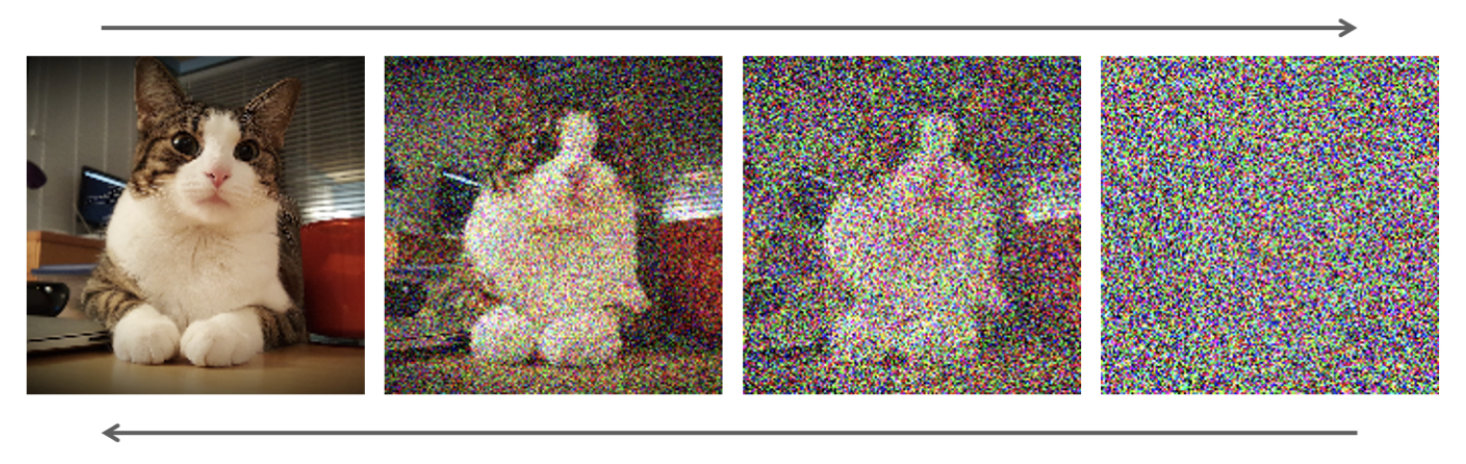
\includegraphics[width = 7in]{\images/DiffSequence}}


\vfill
A diffusion model multi-step (Markovian) VAE where each encoder step adds a small amount of noise.

\slide{Diffusion Model Preview}

Each step of a diffusion model is a VAE:

\vfill
\begin{itemize}
\item $P_\enc(z|y)$ is defined by adding a small amount of noise to $y$.

\vfill
\item $P_\pri(z)$ is trained to model the marginal onto $z$ of $\pop(y)P_\enc(z|y)$.

\vfill
\item A ``denoising'' $\hat{y}_\gen(z)$ is computed by a U-Net.
\end{itemize}

\vfill
Here $z$ contains almost all the information in $y$.

\slide{Fixed Encoder Training}
In a diffusion model the encoder is fixed.

$$\pri^*,\gen^* = \argmin_{\pri,\gen}\;E_{y \sim \pop(y),z \sim \enc(z|y)}\left[-\ln P_\pri(z)P_\gen(y|z)\right]$$

\vfill
This is a cross-entropy loss from a joint ``population distribution'' $P_{\pop,\enc}(y,z)$ to a model
distribution $P_{\pri,\gen}(y,z)$.

\vfill
Assuming universality we get $P_{\pri^*,\gen^*}(z,y) = P_{\pop,\enc}(z,y)$ which implies {\color{red} $P_{\pri^*,\gen^*}(y) = \pop(y)$}.

\slide{Training the Encoder (The Bayesian Interpretation)}

VAEs were originally motivated by a Bayesian interpretation:

\vfill
\begin{itemize}
\item $P_\pri(z)$ is the Bayesian prior on hypothesis $z$.

\vfill
\item $P_\gen(y|z)$ is the propability of the ``evidence'' $y$ given hypothesis $z$.

\vfill
\item $P_\enc(z|y)$ is a model approximating the Bayesian posterior on hypothesis $z$ given evidence $y$.
\end{itemize}

\vfill
The Bayesian motivation is to train $P_\enc(z|y)$ to approximate Bayesian inference.

\slide{Training the Encoder}

$$\enc^*,\pri^*,\gen^* = \argmin_{\enc,\pri,\gen}\;E_{\color{red} y \sim \pop,z\sim P_\enc(z|y)}\;{\cal L}(y,z)$$

\vfill
\begin{eqnarray*}
{\cal L}(y,z) & = & - \ln \frac{P_\pri(z)P_\gen(y|z)}{P_\enc(z|y)}
\end{eqnarray*}

\vfill
Here we can hope to train the encoder to capture a causal origin for $y$.

\slide{Training the Encoder}

{\huge
Consider training $P_\enc$ while holding $P_\pri$ and $P_\gen$ fixed.
\begin{eqnarray*}
  \enc^* & = & \argmin_\enc \;E_{y \sim \pop(y),z \sim \enc(z|y)}\; - \ln \frac{\color{red} P_\pri(z)P_\gen(y|z)}{P_\enc(z|y)} \\
  \\
  & = & \argmin_\enc \;E_{y \sim \pop(y),z \sim \enc(z|y)}\; - \ln \frac{\color{red} P_{\pri,\gen}(y)P_{\pri,\gen}(z|y)}{P_\enc(z|y)} \\
  \\
  &= & \argmin_\enc E_{y \sim \pop(y)} \; {\color{red} KL(P_\enc(z|y),P_{\pri,\gen}(z|y))} + E_{y\sim \pop(y)}\left[-\ln P_{\pri,\gen}(y)\right]
  \end{eqnarray*}

\vfill
Training $P_\enc(z|y)$ to equal $P_{\pri,\gen}(z|y)$ can drive the KL term to zero.

\vfill
Training $P_\pri(z)$ and $P_\gen(y|z)$ can drive the cross-entropy term to $H(\pop)$.
}


\slide{The Evidence Lower Bound (ELBO)}

The previous derivation can be applied to an arbitrary fixed value of $y$ yielding.

\begin{eqnarray*}
\ln P_{\pri,\gen}(y) & \geq  & E_{z \sim P_\enc(z|y)}\; \ln \frac{P_\pri(z)P_\gen(y|z)}{P_\enc(z|y)} \\
\\
& = & E_{z \sim P_\enc(z|y)}\left[-{\cal L}(y,z)\right]
\end{eqnarray*}

\vfill
A Bayesian thinks of $y$ as ``evidence'' for hypothesis $z$ in the Bayesian model.  This method of training $P_\enc(z|y)$ is called {\color{red} variational Bayesian inference}.

\vfill
Under the Bayesian interpretation the negative of the VAE loss is called {\color{red} the evidence lower bound (ELBO)}    .

\slide{Degrees of Freedom}

$$\enc^*,\pri^*,\gen^* = \argmin_{\enc,\pri,\gen}\;E_{\color{red} y \sim \pop,z\sim P_\enc(z|y)}\;{\cal L}(y,z)$$

\vfill
\begin{eqnarray*}
{\cal L}(y,z) & = & - \ln \frac{P_\pri(z)P_\gen(y|z)}{P_\enc(z|y)}
\end{eqnarray*}

\vfill
The objective is fully optimized whenever

\vfill
{\color{red} $$P_\pri(z)P_\gen(y|z) = \pop(y)P_\enc(z_y)$$}

\vfill
Any joint distribution on $(y,z)$ optimizes the bound provided that the marginal on $y$ is $\pop$.

\slide{Posterior Collapse}

Under the Bayesian interpretation we would like $z$ to provide useful information about (a causal origin of) $y$.

\vfill
However the objective function only produces
$$P_\pri(z)P_\gen(y|z) = \pop(y)P_\enc(z|y)$$

\vfill
For language models the generator can assign a meaningful probability to a block of text $y$ independent of $z$.

\vfill
When we train a sentence encoder (a thought vector) as the latent valriable of a language model VAE we can get a constant (zero) thought vector.

\vfill
This is called ``posterior collapse''.

\slide{The Reparameterization Trick}

$$\enc^* = \argmin_{\enc}\;\;E_{y\sim \pop(y),{\color{red} z\sim P_\enc(z|y)}}\;\left[- \ln \frac{P_\pri(z)P_\gen(y|z)}{P_\enc(z|y)}\right]$$

\vfill
Gradient descent on the encoder parameters must take into account the fact that we are sampling from the encoder.

\vfill
To handle this we sample noise $\epsilon$ from a fixed noise distribution and replace $z$ with a determinstc function $z_\enc(y,\epsilon)$

\vfill
$$\enc^*,\pri^*,\gen^* = \argmin_{\enc,\pri,\gen}\;\;E_{y,{\color{red} \epsilon,z=\hat{z}_\enc(y)+\sigma\epsilon}}\;\left[- \ln \frac{P_\pri(z)P_\gen(y|z)}{P_\enc(z|y)}\right]$$

\slide{The Reparameterization Trick}

$$\enc^*,\pri^*,\gen^* = \argmin_{\enc,\pri,\gen}\;\;E_{y,{\color{red} \epsilon,z=\hat{z}_\enc(y)+\sigma\epsilon}}\;\left[- \ln \frac{P_\pri(z)P_\gen(y|z)}{P_\enc(z|y)}\right]$$

\vfill
To get gradients we must have that $\hat{z}_\enc(y)$ is a differentiable function of the encoder parameters.

\vfill
Optimizing the encoder is tricky for discrete $z$.  Discrete $z$ is handled effectively in EM algorithms and general vector quantization (VQ) methods.

\slide{The KL-divergence Optimization}
\vfill
\begin{eqnarray*}
{\cal L}(y) & = & E_{z \sim P_\enc(z|y)}\left[ - \ln \frac{P_\pri(z)P_\gen(y|z)}{P_\enc(z|y)}\right] \\
\\
& = & {\color{red} KL(P_\enc(z|y),P_\pri(z))} + E_{z \sim P_\enc(z|y)}\left[- \ln P_\gen(y|z)\right] \\
\\
\\
&=& {\color{red} \frac{||\hat{z}_\enc(y) - \hat{z}_\pri||^2}{2\sigma^2}} + E_\epsilon\;\frac{||y - \hat{y}_\gen(\hat{z}_\enc(y) + \epsilon)||^2}{2\sigma^2}
\end{eqnarray*}

\vfill
A closed-form expression for the KL term avoids sampling noise.

\slide{EM is Alternating Optimization of the ELBO Loss}

Expectation Maximimization (EM) applies in the (highly special) case where the exact posterior $P_{\pri,\gen}(z|y)$ is samplable and computable.
EM alternates exact optimization of $\enc$ and the pair $(\pri,\gen)$ in:
$$\mbox{VAE:}\;\;\;\;\;\;\; {\color{red} \pri^*,\gen^*} = \argmin_{\color{red} \pri,\gen} \min_{\color{red} \enc} E_{y,\;z \sim P_{\color{red} \enc}(z|y)}\;\;- \ln \frac{P_{\color{red} \pri,\gen}(z,y)}{P_{\color{red} \enc}(z|y)}$$

\vfill
$$\mbox{EM:}\;\;\;\;\;\; {\color{red} \pri^{t+1},\gen^{t+1}} =  \argmin_{\color{red} \pri,\gen}\;\;\;\;E_{y,\;z \sim P_{\color{red} \pri^t,\gen^t}(z|y)}\; - \ln P_{\color{red} \pri,\gen}(z,y)$$

\vfill
\centerline{\hspace{1em} Inference \hspace{6em} Update \hspace{2.5em}~}
\centerline{(E Step) \hspace{6em} (M Step) ~}
\centerline{ $P_\enc(z|y) = P_{\pri^{\color{red} t},\gen^{\color{red} t}}(z|y)$ \hspace{2.5em} Hold $P_\enc(z|y)$ fixed \hspace{0em}~}

\slide{END}

\end{document}
